\documentclass[11pt]{article}
\usepackage[margin=1in]{geometry}
\usepackage{amsmath,amssymb}
\usepackage{booktabs}
\usepackage{graphicx}
\usepackage{array}
\usepackage{float}
\usepackage{url}

\newcolumntype{L}[1]{>{\raggedright\arraybackslash}p{#1}}
\emergencystretch=2em

\title{Two-Step Contextual Enrichment with Hyper-Dimensional Anchors:\\Discrete Control Prefixes for Inference-Time Reliability}
\author{Kaleb Cadenhead\\Automation Optimization\\\texttt{kcadenhead@automationoptimization.com}}
\date{\today}

\newcommand{\tsce}{\textsc{TSCE}}
\newcommand{\hda}{\textsc{HDA}}
\newcommand{\hdalong}{Hyper-Dimensional Anchor}

\begin{document}
\maketitle

\begin{center}
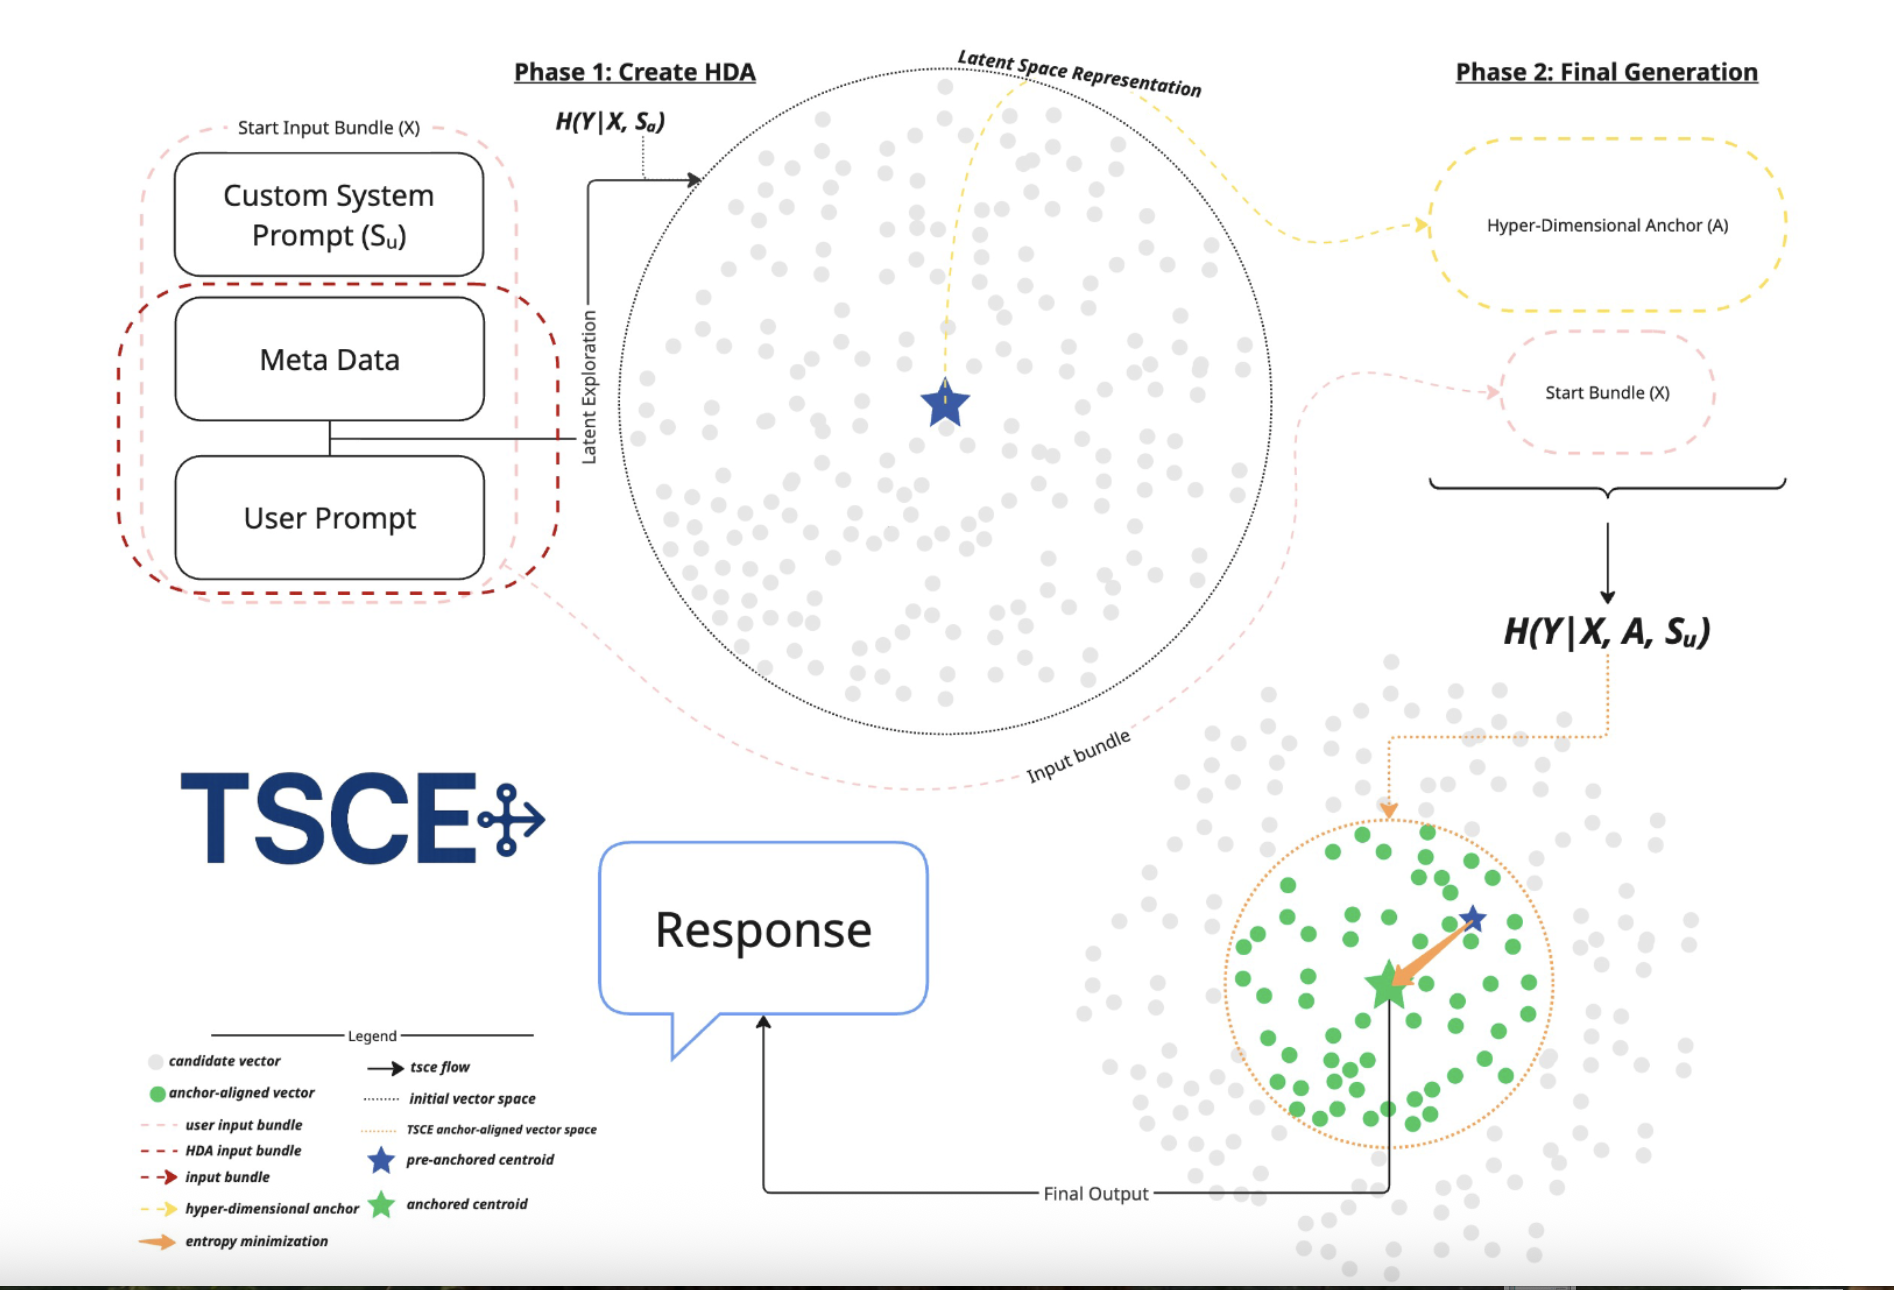
\includegraphics[width=0.92\linewidth]{figures/tsce/tsce_graphic.png}
\end{center}

\begin{abstract}
Many language-model failures begin before the first visible token: the model starts decoding from the wrong conditional state. Two-Step Contextual Enrichment (\tsce) is a discrete inference-time control method for improving reliability without changing model weights. It first generates a \hdalong{} (\hda), then decodes the final answer under that anchor. The \hda{} is the steering prefix under test: an ordinary input-token sequence selected to shift the model's pre-decode state into a better task basin before visible answer generation.

Operationally, \tsce{} is a wrapper around existing chat-completion calls. It adds an anchor-generation step and a small final-prompt control prefix, without model retraining or activation-patching infrastructure. This makes the deployment cost explicit: one extra anchor call when anchors are generated online, plus ordinary prompt-token overhead during the final decode.

Across 17 comparable black-box evaluations, the paired baseline-vs-best summary improves from $2093/3330$ solved instances ($62.9\%$) to $2736/3330$ solved instances ($82.2\%$), with 10,460 condition-level scored outputs across 64 pass-rate rows. This is an upper-envelope run-level summary across heterogeneous \hda{} policies, not a single frozen recipe. A separate 100-task fixed-policy Gemma validation with compact \texttt{latent\_bias} anchors is neutral: baseline and \tsce{} both solve $66/100$ tasks. On 69 Gemma prompts selected because baseline decoding failed, a 14,421-row format-robustness sweep shows that several noncanonical \hda{} surface forms still rescue many failures, while removing the final-answer scaffold largely collapses the effect.

In a controlled token-causality evaluation, task-relevant \hda{} strings lift the target-vs-distractor pre-generation probe margin by $+1.1629$, while tokenizer-matched random controls remain near zero ($-0.0593$, $-0.0011$, $-0.0231$). A naturalistic story-theme probe shows the same measurement pattern for \emph{forgiveness after betrayal}: controlled theme-proxy \hda{} strings lift the pre-generation margin by $+2.5849$, while matched random controls do not. A larger result corpus supports anchor generation, policy development, and mechanistic diagnostics; its inventory is separated from accuracy claims in Appendix A.
\end{abstract}

\section{Introduction}

\tsce{} is a discrete inference-time control method. It treats ordinary input tokens as a control interface, not merely as text for instruction following. The \hda{} is the causal steering prefix under test: a compact token sequence generated before the final answer and used to move the model's pre-decode state into a more useful task basin.

Language-model failures often begin before the first visible token is emitted. A model may have the relevant capability but enter the final decode in a broad, weakly constrained region of its conditional distribution. In that state, repeated samples drift, formatting constraints are missed, and small prompt ambiguities become large output differences. This framing is consistent with the prompt sensitivity observed in few-shot language models and with the practical difficulty of evaluating free-form model outputs reliably \cite{few-shot,fair-evaluators}.

\tsce{} addresses that failure mode by inserting a learned or sampled token intervention before the final answer. The intervention is the \hda{}. Its role is not to explain the task to a human. Its role is to bias the model's internal trajectory so that the final decode starts from a narrower and more task-appropriate region.

This paper evaluates the following claim:
\begin{quote}
\tsce{} improves reliability when the \hda{} shifts the model's pre-decode state into a better task basin.
\end{quote}

The evaluation is organized around three forms of evidence. First, outcome benchmarks measure downstream reliability under \tsce{} conditioning. Second, controlled token-causality tests measure target-relevant probability movement before long-form generation. Third, proxy-family and activation-space diagnostics characterize which token neighborhoods produce the measured shift. The limitations section bounds the claim to cases in which the \hda{} produces task-relevant pre-decode movement.

\section{Method}

Let $X$ be the user prompt, $A$ be the \hda{} token sequence, and $Y$ be the final answer. \tsce{} has two phases:
\begin{align}
    A &\sim P_{\phi}(A \mid X, S_{\mathrm{anchor}}), \\
    Y &\sim P_{\theta}(Y \mid X, A, S_{\mathrm{final}}).
\end{align}

The method is model-agnostic because $A$ is passed through the same token interface as any other prompt prefix. No weights are changed and no hidden activations are patched by hand. The intervention still has a latent effect because every token is embedded, attended to, and transformed into high-dimensional hidden state before decoding. This places \tsce{} near work on code-based neurosymbolic reasoning, adversarial gibberish-prompt effects, latent-action control, and continuous-latent reasoning, but only as neighboring design context. Those sources motivate the plausibility of token-mediated or representation-mediated control; the evidence for \tsce{} itself is the outcome and pre-decode measurement reported below \cite{code-anchoring,gibberish-prompts,latent-actions,coconut,compressed-cot}.

\subsection{Operational Deployment Profile}

The practical deployment shape is intentionally simple. \tsce{} can be inserted as a two-call wrapper around an existing chat-completion pipeline: phase 1 generates or retrieves an \hda{}, and phase 2 sends the original request with the \hda{} placed in the final conditioning context. The runtime cost is explicit: one additional anchor-generation call when anchors are generated online, plus the token overhead of the \hda{} and fixed scaffold in the final prompt. If anchors are precomputed, cached, or supplied by an external policy, the integration reduces to a single final call with a control prefix.

The reference Python implementation includes a \texttt{TSCEChat} wrapper in \path{tsce_agent_demo/tsce_chat.py}. The wrapper accepts either a plain string prompt or an OpenAI-style chat message array, supports OpenAI, Azure OpenAI, Ollama, and a local phase-2 backend path, and records phase-level request, response, usage, and latency metadata for operational logging. It can also accept \texttt{force\_anchor}, which allows a separate anchor service or learned policy to be dropped in without changing the final-answer application code. The implementation lineage has been used by Automation Optimization since 2023 in applied automation work; that operational history motivates the wrapper design, while the benchmark and causality claims in this paper remain limited to the measured artifacts reported below.

The intended adoption pattern is an A/B test around existing prompts, not a replacement for the surrounding reliability stack. \tsce{} is most relevant when failures look like underconstrained decoding, format drift, or brittle instruction adherence. In those cases, teams can compare baseline, \tsce{}, and matched controls while directly measuring added tokens, latency, and task-level acceptance rates.

\subsection{HDA Generation Policy}

The evidence in this paper uses two distinct \hda{} sources. First, the black-box reliability subset contains heterogeneous runs: some use sampled prompt-family anchors, some use generated or searched anchors, and some evaluate multiple \tsce{}/\hda{} variants. For that reason the paired baseline-vs-best result is an upper-envelope run summary. It asks whether each run contained a \tsce{}/\hda{} condition that produced the predicted reliability shift; it should not be read as the performance of a single fixed production recipe.

Second, newer Gemma evaluations use a reproducible prompt-family policy. The phase-1 model samples multiple candidate anchors from one or more prompt families: \texttt{opaque\_control}, \texttt{latent\_bias}, \texttt{task\_abstract}, and \texttt{keyboard\_drift}. The default family is \texttt{latent\_bias}. Candidates are canonicalized as \texttt{<HDA>...</HDA>} strings and selected by a heuristic score that favors compact alphabetic tokens, high uniqueness, low repetition, low overlap with the user prompt, absence of digits or punctuation, absence of instruction vocabulary, and low sentence-likeness. This draws on the same premise as control-code conditioning and pause-token delayed computation: pre-output tokens can change the distribution and computation used for the following decode \cite{control-codes,pause-tokens}. The Gemma comparison path records the prompt family, selector, candidate count, selected candidate, candidate features, source mode, anchor temperature, and top-$p$ in each run. Default sampling uses anchor temperature $1.25$, top-$p=0.95$, and the heuristic selector; final answer decoding is run at low temperature where deterministic comparison is required.

This policy description is separate from learned \hda{} policies. Diffusion and reinforcement-learning policies are engineering routes for discovering better anchors, but the mechanism claim only requires an ordinary-token prefix that produces measurable pre-decode movement. Appendix~\ref{app:hda-policies} gives the policy summary used for reproduction.

\subsection{Terminology and Related Methods}

The term \hdalong{} is literal.
\begin{itemize}
    \item It is an \emph{anchor} because it pulls the second pass toward a region of behavior before the answer begins.
    \item It is \emph{hyper-dimensional} because the steering effect is mediated through the model's embedding, attention, and residual-stream geometry rather than through a single human-readable instruction.
    \item It is a \emph{token sequence} because \tsce{} uses ordinary input tokens as the control channel.
\end{itemize}

\tsce{} is related to prior work on control prefixes and latent control, but the intended distinction is functional: \tsce{} uses ordinary tokens as a control prefix optimized for internal steering, not as a human-readable explanation or final-answer draft. The closest prior work provides analogies and boundary cases rather than direct validation: code-based neurosymbolic reasoning shows that non-natural-language structure can support reasoning, adversarial gibberish-prompt work shows that semantically odd strings can affect model behavior, and latent-action or continuous-latent methods show related ways of biasing computation through compact internal representations \cite{code-anchoring,gibberish-prompts,latent-actions,coconut,compressed-cot}.

\begin{figure}[H]
    \centering
    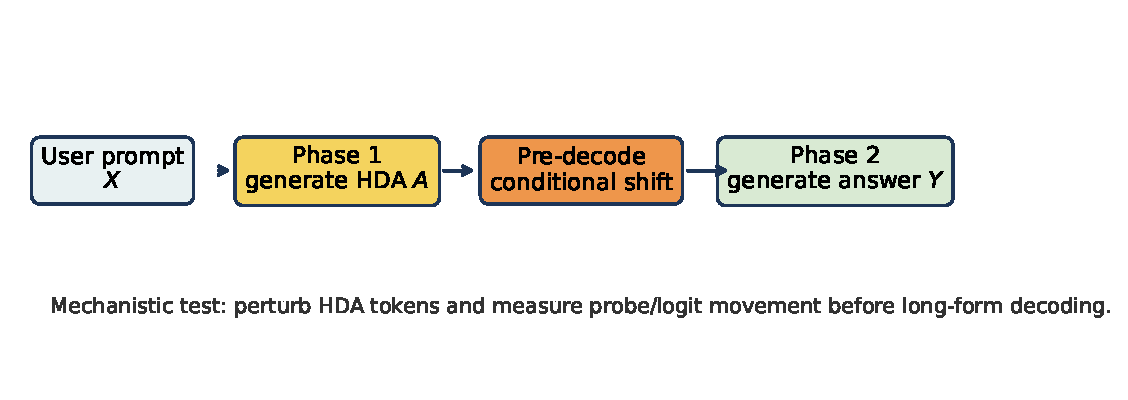
\includegraphics[width=0.92\linewidth]{figures/tsce/figure1_token_intervention.pdf}
    \caption{The \hda{} is the proposed mediator in \tsce{}: it is generated before the visible answer and shifts the model's pre-decode state through the normal token pathway.}
    \label{fig:token-intervention}
\end{figure}

\section{Hypotheses}

The mechanism implies five testable hypotheses.

\begin{enumerate}
    \item \textbf{Outcome lift:} conditioning on \hda{} strings should improve task reliability when the \hda{} moves the model toward useful constraints.
    \item \textbf{Pre-decode movement:} the effect should be measurable before long-form generation, not only after grading final answers.
    \item \textbf{Matched controls:} tokenizer-matched random strings should not reproduce the same target-relevant movement.
    \item \textbf{Surface-form robustness:} some effect should survive non-semantic perturbations of an effective \hda{}---including shuffling, deletion, wrapper changes, line breaks, and tag changes---when the modified sequence remains in a similar conditioning basin.
    \item \textbf{Compositionality:} semantically relevant proxy neighborhoods should move the model more than neutral or irrelevant token neighborhoods.
\end{enumerate}

The experiments below are organized around these hypotheses.

\section{Outcome Evaluation}

Black-box task evaluations estimate the downstream effect of \hda{} conditioning on final-answer accuracy. Each evaluation compares a baseline condition against one or more \tsce{}/\hda{} conditions. Table~\ref{tab:outcome} shows a 300-task GPT-3.5 evaluation that includes single-pass, Chain-of-Thought, Self-Refine, and \tsce{}-conditioned variants. These comparison points represent verbal and agentic test-time scaffolds rather than hidden control prefixes \cite{cot,self-consistency,self-refine,react}.

\begin{table}[H]
\centering
\begin{tabular}{lcc}
\toprule
Method & Passes & Pass rate \\
\midrule
Baseline & 147/300 & 49.0\% \\
Chain-of-Thought & 186/300 & 62.0\% \\
Self-Refine & 163/300 & 54.3\% \\
\tsce{} & 238/300 & 79.3\% \\
CoT+\tsce{} & 240/300 & 80.0\% \\
Refine+\tsce{} & 242/300 & 80.7\% \\
\bottomrule
\end{tabular}
\caption{Outcome-level reliability on the 300-task GPT-3.5 evaluation. The \tsce{}-conditioned conditions outperform the corresponding non-\tsce{} baselines, indicating that \hda{} conditioning contributes reliability beyond the additional inference pass alone.}
\label{tab:outcome}
\end{table}

\begin{figure}[H]
    \centering
    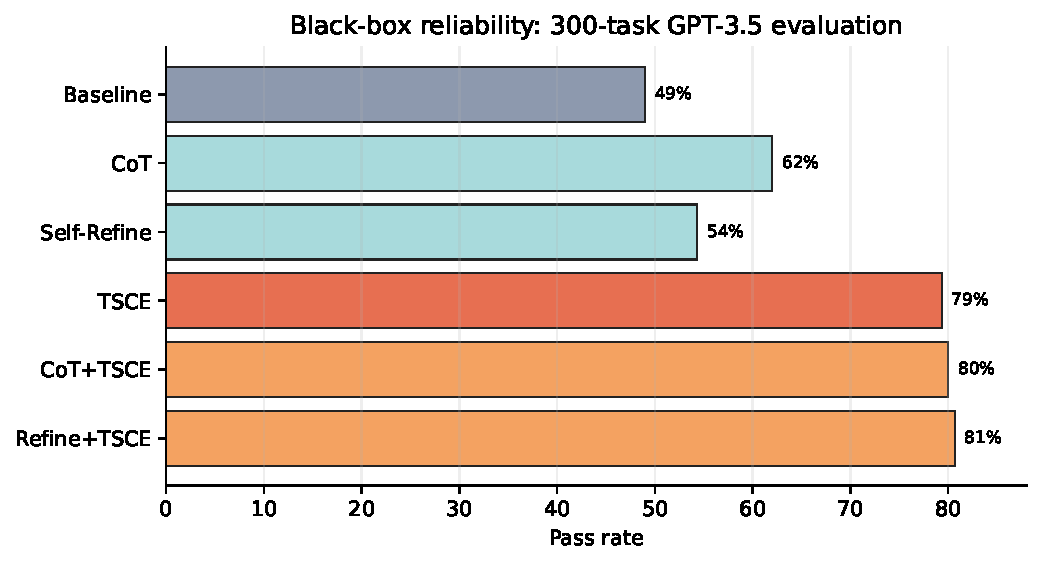
\includegraphics[width=0.86\linewidth]{figures/tsce/figure2_behavioral_pass_rates.pdf}
    \caption{Outcome-level pass rates for the 300-task GPT-3.5 evaluation.}
    \label{fig:outcome}
\end{figure}

The comparable black-box reliability subset contains 17 run-level evaluations that include pass counts for a baseline and at least one \tsce{}/\hda{} condition. Across all pass-rate rows, this subset contains 64 condition rows and 10,460 condition-level scored outputs. The aggregate baseline-vs-best comparison is a paired run-level upper-envelope summary: it selects one baseline row and one best \tsce{}/\hda{} row per run, producing a 3,330-instance denominator on each side of the comparison. Under that paired summary, baseline conditions solve $2093/3330$ instances ($62.9\%$), while the best \tsce{}/\hda{} condition within each run solves $2736/3330$ instances ($82.2\%$). Because run configurations, model settings, task slices, and \hda{} generation policies are not identical, this is framed as a cross-run reliability summary rather than as an independence-weighted meta-analysis or a fixed-policy replication result. The behavioral pattern is consistent with the proposed mechanism: 15 of 17 run-level evaluations show positive lift, 12 of 17 show at least $+15$ percentage points, and the median best-condition lift is $+22.0$ percentage points.

\begin{table}[H]
\centering
\begin{tabular}{L{0.68\linewidth}r}
\toprule
Cross-run measure & Value \\
\midrule
Run-level black-box evaluations & 17 \\
Pass-rate condition rows & 64 \\
Condition-level scored outputs & 10,460 \\
Paired baseline-vs-best task instances & 3,330 per side \\
Aggregate baseline accuracy over paired instances & 2093/3330 (62.9\%) \\
Aggregate best \tsce{}/\hda{} accuracy over paired instances & 2736/3330 (82.2\%) \\
Evaluations with positive lift & 15/17 \\
Evaluations with lift $\geq 15$ percentage points & 12/17 \\
Median best-condition lift & +22.0 percentage points \\
\bottomrule
\end{tabular}
\caption{Cross-run summary of black-box evaluations. Best-condition aggregation asks whether any \tsce{}/\hda{} configuration in each run produced the predicted downstream reliability shift. It is an upper-envelope summary across heterogeneous setups; fixed-policy replication should report each chosen \hda{} generation policy separately rather than selecting the best condition after evaluation.}
\label{tab:cross-run-outcome}
\end{table}

To check the cherry-picking risk directly, we also ran a fixed-policy Gemma validation. The policy was selected before evaluation: Gemma E4B, task kind \texttt{auto}, 100 generated tasks, seed 260426, \texttt{latent\_bias} anchor family, heuristic source mode, heuristic selector, two anchor candidates, compact 4--8 token anchors, anchor temperature $1.25$, top-$p=0.95$, and final-answer temperature $0.01$. This fixed policy does not reproduce the upper-envelope lift. \tsce{} ties the baseline at $66/100$, with four \tsce{}-only wins and four baseline-only wins. The matched opaque controls are also close: random-valid anchors solve $65/100$, shuffled anchors solve $64/100$, and context-collision anchors solve $66/100$. This run disables activation capture, so it is an outcome-only fixed-policy check. The result is useful precisely because it is negative: the upper-envelope summary shows that some \hda{} policies can help, but this compact fixed policy does not by itself establish fixed-recipe outcome improvement.

\begin{table}[H]
\centering
\begin{tabular}{lcc}
\toprule
Condition & Passes & Pass rate \\
\midrule
Baseline & 66/100 & 66.0\% \\
Readable control & 64/100 & 64.0\% \\
\tsce{} compact \texttt{latent\_bias} & 66/100 & 66.0\% \\
Random-valid matched anchor & 65/100 & 65.0\% \\
Shuffled anchor & 64/100 & 64.0\% \\
Context-collision anchor & 66/100 & 66.0\% \\
\bottomrule
\end{tabular}
\caption{Fixed-policy Gemma validation on a 100-task auto slice. Unlike the baseline-vs-best summary, this table freezes one compact \hda{} policy before evaluation and reports all matched controls.}
\label{tab:fixed-policy-gemma}
\end{table}

\subsection{Format Robustness on Baseline Failures}

The fixed-policy result above asks whether one compact \hda{} recipe improves a mixed 100-task slice. A separate format-robustness sweep asks a narrower question: when baseline decoding already fails, is the effect tied to one exact \texttt{<HDA>... </HDA>} surface form? We evaluated Gemma E4B on 69 prompts selected from baseline failures, using 16 candidate anchors per prompt, 13 \hda{} format variants, and an empty-system baseline. Final-answer decoding used temperature $0.01$ and top-$p=0.95$, producing 14,421 scored rows.

\begin{table}[H]
\centering
\begin{tabular}{lccc}
\toprule
Condition & Passes & Pass rate & Oracle@16 \\
\midrule
Baseline empty system & 0/69 & 0.0\% & -- \\
One token per line & 614/1104 & 55.6\% & 65.2\% \\
User prefix & 599/1104 & 54.3\% & 63.8\% \\
Control tag & 540/1104 & 48.9\% & 52.2\% \\
Canonical inline & 534/1104 & 48.4\% & 55.1\% \\
User suffix & 513/1104 & 46.5\% & 58.0\% \\
Multi-block \hda{} & 512/1104 & 46.4\% & 53.6\% \\
System no scaffold & 53/1104 & 4.8\% & 24.6\% \\
\bottomrule
\end{tabular}
\caption{Gemma E4B format-robustness sweep on 69 baseline-failure prompts. Multiple noncanonical \hda{} surface forms preserve substantial rescue, while placing the anchor in the system message without the final-answer scaffold largely collapses the effect.}
\label{tab:format-robustness}
\end{table}

This separates payload robustness from scaffold invariance. The result argues against the narrow explanation that \tsce{} only found a brittle XML-like prompt trick: line-wrapped, control-tagged, user-prefixed, and multi-block variants all preserve substantial rescue. At the same time, the weak \texttt{system\_no\_scaffold} condition shows that the anchor is not an arbitrary string that works wherever it is placed. The \hda{} must be consumed in a conditioning context that influences the final decode.

We distinguish comparable accuracy trials from supporting generation, policy, and mechanistic artifacts. The broader result tree contains 479 files and 100,816 counted rows/records/log lines; detailed accounting is provided in Appendix~\ref{app:result-corpus}.

\begin{figure}[H]
    \centering
    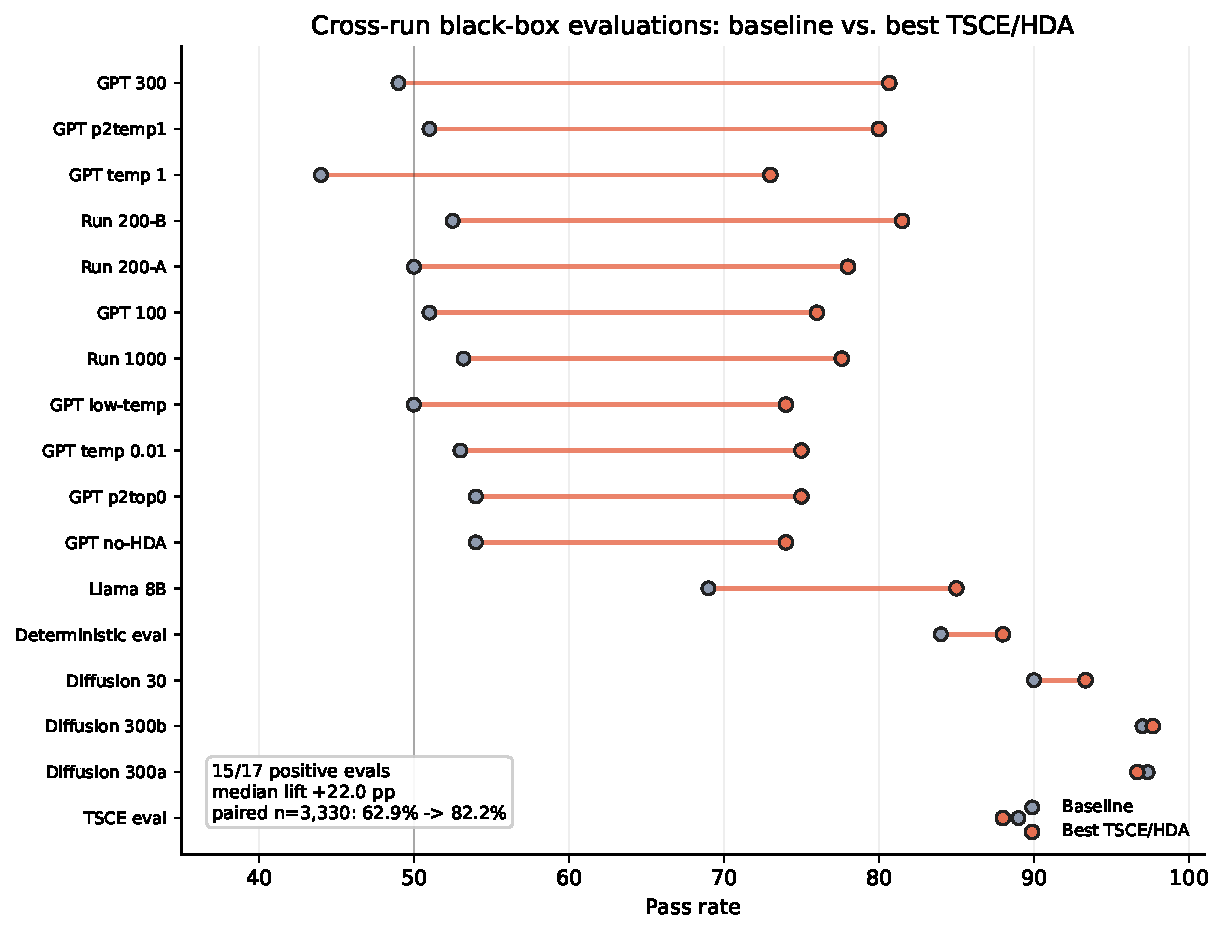
\includegraphics[width=0.98\linewidth]{figures/tsce/figure7_cross_run_lifts.pdf}
    \caption{Cross-run black-box evaluation summary. Most run-level evaluations show positive lift from baseline to the best \tsce{}/\hda{} condition; high-ceiling evaluations show smaller or neutral effects when baseline performance is already near saturation or when the \hda{} does not produce a beneficial pre-decode shift.}
    \label{fig:cross-run-lifts}
\end{figure}

The variation across evaluations is relevant to the mechanism rather than incidental. \tsce{} is expected to improve reliability when the generated \hda{} moves the model toward task-relevant constraints, and to produce smaller gains when the model, task, or anchor-generation procedure does not create a useful pre-decode shift. That distinction also separates the present evidence from majority-vote or search-heavy test-time compute methods, which can improve outcomes through additional sampling, acting, or refinement rather than through a measured pre-decode control state \cite{self-consistency,self-refine,react}.

\section{Controlled Token-Causality Evaluation}

The controlled token-causality evaluation tests the proposed mediator directly. A held-out composite target phrase is used as the target concept:
\begin{center}
\emph{a greenhouse full of sleeping glass birds}
\end{center}

The \hda{} is constrained not to name the target phrase. Instead, controlled \hda{} strings are constructed from indirect proxy families: glass/light, avian/sky, garden/green, and sleep/quiet. The measured variable is a pre-generation target-vs-distractor probe margin, defined as target probe log-probability minus negative subject probe log-probability. Because this quantity is measured before long-form generation, it tests the pre-decode state rather than post hoc answer quality.

\begin{table}[H]
\centering
\begin{tabular}{lcc}
\toprule
Condition & Mean margin & Lift vs. no \hda{} \\
\midrule
No \hda{} & -3.7140 & 0.0000 \\
\hda{} & -2.5511 & +1.1629 \\
Shuffled \hda{} & -2.7742 & +0.9398 \\
Head-deleted \hda{} & -2.8808 & +0.8332 \\
Mid-deleted \hda{} & -2.6698 & +1.0441 \\
Tail-deleted \hda{} & -2.6374 & +1.0766 \\
Neutral-replaced \hda{} & -2.8363 & +0.8777 \\
Random matched 1 & -3.7733 & -0.0593 \\
Random matched 2 & -3.7151 & -0.0011 \\
Random matched 3 & -3.7371 & -0.0231 \\
\bottomrule
\end{tabular}
\caption{Controlled token-causality conditions. Task-relevant \hda{} strings move the pre-decode target margin, while tokenizer-matched random strings remain near the no-\hda{} baseline.}
\label{tab:token-causality}
\end{table}

\begin{figure}[H]
    \centering
    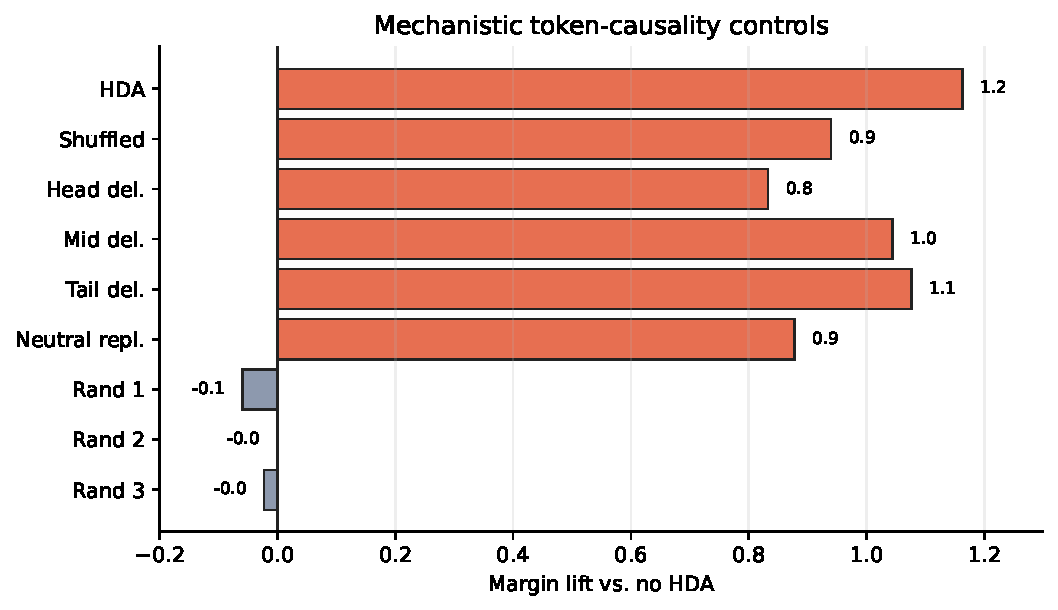
\includegraphics[width=0.90\linewidth]{figures/tsce/figure3_greenhouse_condition_lifts.pdf}
    \caption{Pre-generation probe-margin lift under controlled \hda{} perturbations.}
    \label{fig:token-causality}
\end{figure}

The result supports the mediator role assigned to the \hda{}. The controlled \hda{} condition increases the pre-generation margin by $+1.1629$ relative to no-\hda{}, while three tokenizer-matched random controls produce lifts near zero. This separates task-relevant token steering from the mere presence of additional prefix text. Under the proposed mechanism, reliability improves when this pre-decode movement shifts probability mass toward outputs that better satisfy the task. In information-theoretic terms, conditioning on an informative variable reduces uncertainty in expectation; this is the narrow sense in which the anchor acts as an entropy-reducing intervention before the final sample is drawn \cite{information-theory}.

\subsection{Naturalistic Theme Probe}

The greenhouse target is deliberately artificial: it gives strong experimental control, but it is not representative of everyday task semantics. To test whether the same probe construction extends to a more natural concept, a second token-causality evaluation uses the story theme \emph{forgiveness after betrayal}. The positive probes include the exact theme, the facets forgive, betray, and trust, and a narrative-frame probe. Negative probes are other story themes: homecoming after exile, memory as inheritance, and freedom purchased by sacrifice.

\begin{table}[H]
\centering
\begin{tabular}{lcc}
\toprule
Condition & Mean margin & Lift vs. no \hda{} \\
\midrule
No \hda{} & -0.3342 & 0.0000 \\
\hda{} & 2.2507 & +2.5849 \\
Shuffled \hda{} & 2.1973 & +2.5314 \\
Context-collision \hda{} & -0.3485 & -0.0144 \\
Random matched 1 & -0.8837 & -0.5496 \\
Random matched 2 & -0.4713 & -0.1372 \\
Random matched 3 & -0.1162 & +0.2180 \\
\bottomrule
\end{tabular}
\caption{Naturalistic theme token-causality evaluation for \emph{forgiveness after betrayal}. Controlled theme-proxy \hda{} strings move the pre-decode margin toward the target theme, while context-collision and tokenizer-matched random controls do not reproduce the effect.}
\label{tab:naturalistic-token-causality}
\end{table}

This result is not a substitute for broad natural-task validation, but it addresses the main concern raised by the artificial greenhouse target: the same pre-generation probe trick can detect target-relevant movement for a natural story theme. The effect is also directionally specific. The controlled \hda{} lift is $+2.5849$, shuffled anchors preserve most of the movement, the context-collision control is essentially unchanged from no-\hda{}, and matched random controls do not produce a comparable lift.

\section{Proxy-Family Structure}

The controlled perturbations clarify which properties of the \hda{} are relevant to the observed effect.

First, the effect is not caused by arbitrary prefix text. Tokenizer-matched random strings produce near-zero lift, indicating that the token sequence must land in a useful region of the model's conditional space.

Second, the effect is not tied to one exact surface form. Shuffled and deletion variants preserve much of the lift, implying an equivalence class of useful token sequences whose different surface forms can activate a similar semantic basin.

The baseline-failure format sweep in Table~\ref{tab:format-robustness} supports the same interpretation at the downstream task level: several surface realizations of the same candidate anchor payload remain effective, while removing the final-answer scaffold can destroy most of the effect.

Third, the effect is compositional. With total proxy-token budget fixed, proxy-family coverage helps, but composition matters. Coverage across all four target families gives mean lift $+1.9312$, while the glass/light + avian/sky pair gives $+2.2404$. Family-presence deltas identify the strongest neighborhoods for this target as glass/light $+0.7247$ and avian/sky $+0.7078$, followed by garden/green $+0.3247$ and sleep/quiet $+0.1412$.

\begin{figure}[H]
    \centering
    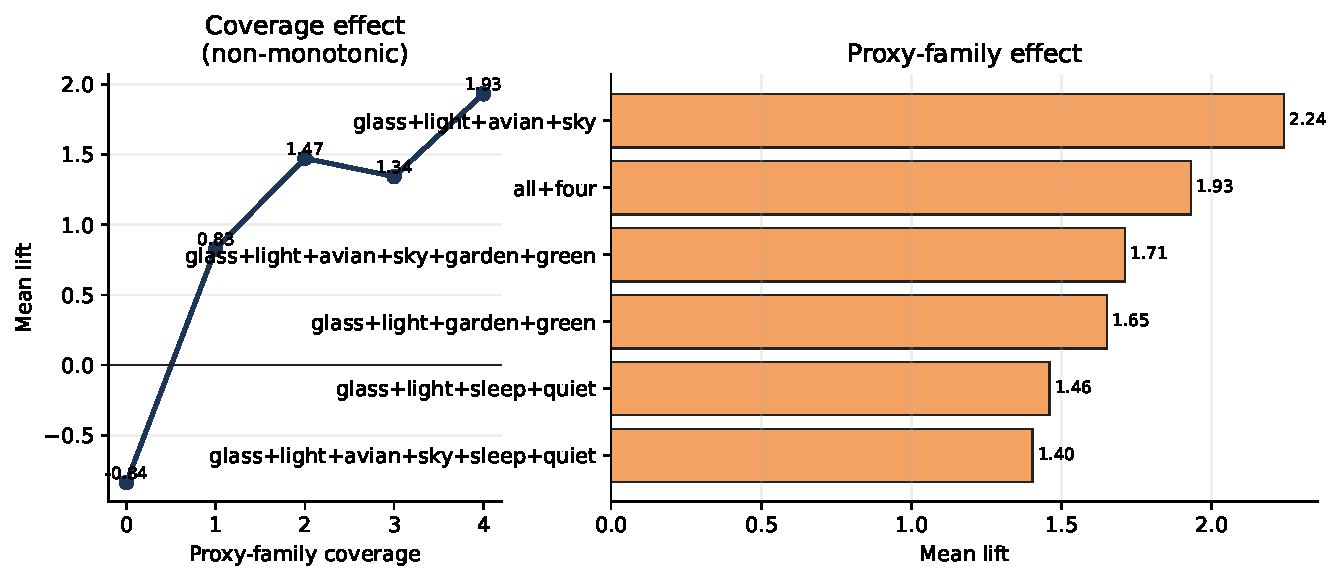
\includegraphics[width=0.96\linewidth]{figures/tsce/figure4_proxy_family_effects.pdf}
    \caption{Proxy-family geometry. Coverage contributes to lift, but the strongest effect comes from proxy neighborhoods that best match the target basin.}
    \label{fig:proxy-family}
\end{figure}

The resulting interpretation is that an effective \hda{} is a compact hard-token attractor: a discrete prefix whose value comes from composed token evidence that moves the model into a useful high-dimensional basin. The comparison to compact latent or embedding-space representations is an analogy for the kind of movement being measured, not evidence that \hda{} strings inherit the guarantees or mechanisms of those methods \cite{vec2vec,latent-actions,coconut}.

\section{Activation-Space Diagnostics}

The same claim can be represented geometrically. Without an \hda{}, the model begins decoding from a broad conditional region. A useful \hda{} moves the pre-decode state toward a task-relevant basin; a tokenizer-matched random string is not expected to make the same directed move. Figure~\ref{fig:latent-basin} is a conceptual visualization of this mechanism, not a substitute for the measured evaluations above.

\begin{figure}[H]
    \centering
    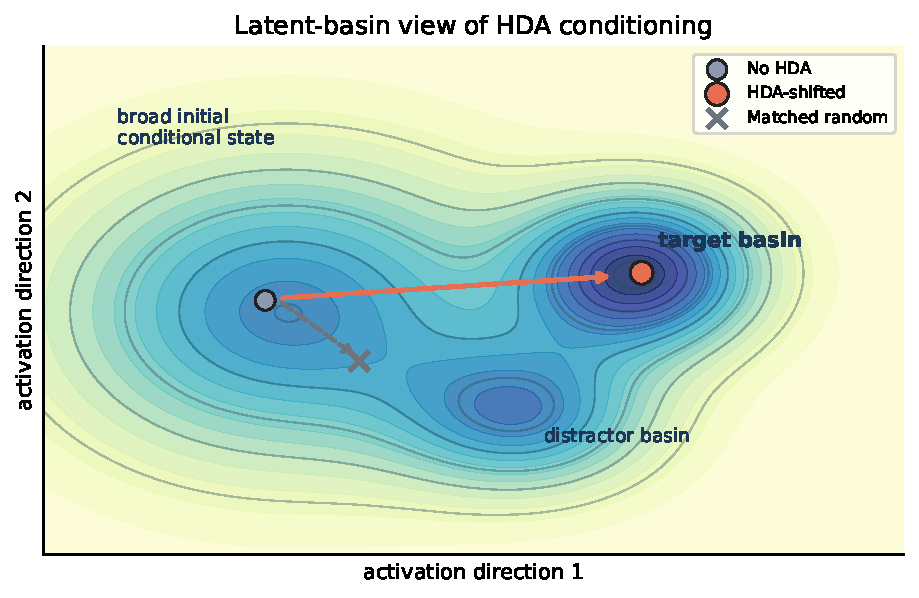
\includegraphics[width=0.88\linewidth]{figures/tsce/figure5_latent_basin_schematic.pdf}
    \caption{Conceptual activation-space view. The \hda{} is useful when it moves the pre-decode state toward a target basin before the final answer is sampled.}
    \label{fig:latent-basin}
\end{figure}

Activation-space diagnostics from Gemma latent-zone evaluations provide an additional internal measurement. In the symbolic-transform diagnostic, class-vector alignment separates in later layers: the good-\hda{} alignment exceeds the control alignment by $+0.0839$ at layer 40 and $+0.0886$ at layer 41. These diagnostics are supportive rather than dispositive: the proposed mechanism predicts that effective \hda{} prefixes should leave a measurable trace in hidden-state geometry before or during the controlled decode. The diagnostic role is similar in spirit to embedding-space translation and latent-action work, but the citation is used only to situate the representation-movement framing; the TSCE-specific claim rests on the matched-control measurements in this paper \cite{vec2vec,latent-actions}.

\begin{figure}[H]
    \centering
    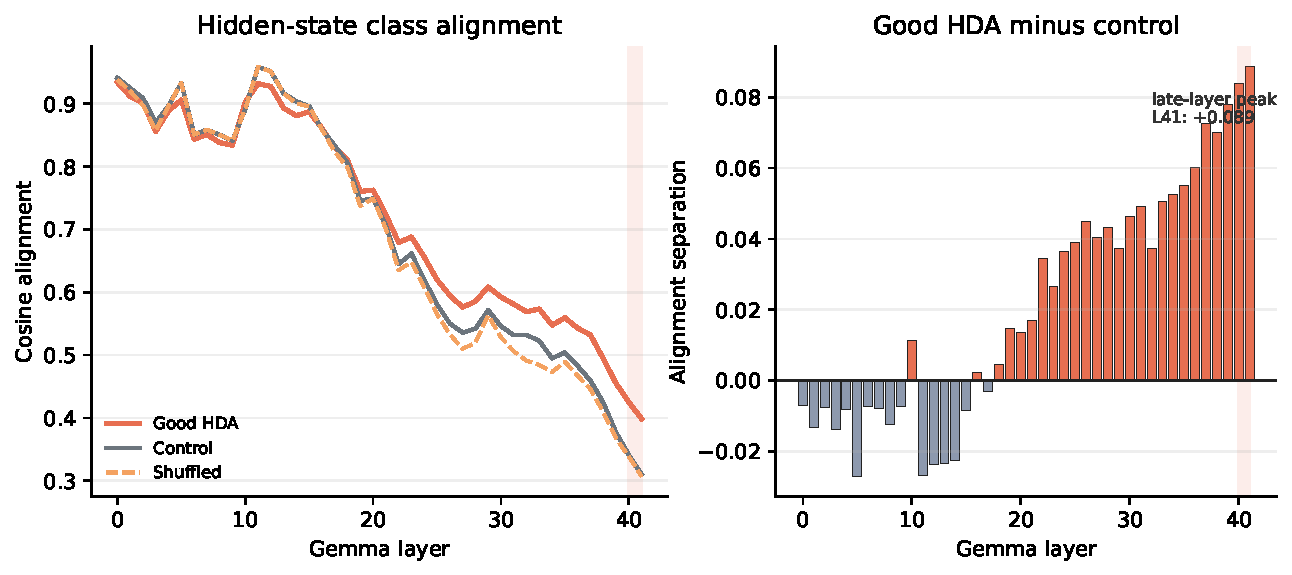
\includegraphics[width=0.96\linewidth]{figures/tsce/figure6_activation_layer_separation.pdf}
    \caption{Activation-space diagnostic from a Gemma latent-zone evaluation. Good-\hda{} class alignment separates from controls in late layers, consistent with a token-mediated hidden-state shift.}
    \label{fig:activation-separation}
\end{figure}

\section{Scope and Limitations}

The claim is bounded in eight ways.

\begin{itemize}
    \item \tsce{} does not show that hard-token \hda{} strings are as expressive as arbitrary continuous activation edits.
    \item \tsce{} does not require vector patching to work. Vector patching tests whether a detached mean activation delta can replace the token pathway; \tsce{} claims only token-mediated conditioning through the normal model interface.
    \item The baseline-vs-best outcome summary is an upper-envelope view across heterogeneous configurations, not a single fixed \hda{} generation recipe. The fixed compact Gemma \texttt{latent\_bias} validation in Table~\ref{tab:fixed-policy-gemma} is neutral, so the present outcome evidence should not be read as proving a ready fixed production policy.
    \item The current \hda{} generation policy is reproducible, but not claimed to be optimal. Learned diffusion and reinforcement-learning policies remain separate engineering extensions.
    \item \tsce{} does not imply that every opaque string is useful. Random matched strings fail in the mechanistic test.
    \item Surface-form robustness does not imply scaffold invariance. The \hda{} must still be placed in a conditioning context that the model uses before answer decoding.
    \item \tsce{} does not imply that proxy coverage is monotonic. Coverage contributes to lift, but family geometry matters.
    \item \tsce{} does not guarantee uniform gains across all models and tasks. The expected benefit depends on whether the \hda{} produces useful pre-decode movement.
    \item \tsce{} is not benchmarked here against the latest agentic scaffolds, search-heavy agents, or broader test-time compute methods \cite{self-consistency,self-refine,react}.
\end{itemize}

These limitations are part of the proposed mechanism. The claim does not require every \hda{} or every geometry diagnostic to succeed. It requires a link between outcome lift and a measurable pre-decode intervention, and the controlled token-causality evaluation supplies direct evidence for that link. Responsible deployment also requires standard provenance, access-control, and monitoring practices for generated control strings, consistent with broader system-card guidance for deployed language models \cite{gpt4-system-card}.

\section{Conclusion}

\tsce{} is a two-step control procedure: the first step generates a \hdalong{}, and the second step decodes the final answer under that anchor. The proposed mechanism is that reliability improves when the \hda{} shifts the model into a more task-appropriate pre-decode region.

The black-box evaluations measure the downstream effect. The controlled token-causality evaluation measures the proposed mediator: task-relevant \hda{} strings shift pre-generation probe margins while matched random strings do not. Together, these results support a discrete-control-prefix account of \hda{} conditioning.

The neutral fixed-policy Gemma run is part of the conclusion, not an exception to hide. Some anchor policies produce large effects; others are neutral. This makes the practical claim narrower and more useful. \tsce{} should be read as a framework for discovering and validating control prefixes, not as a one-size-fits-all recipe.

For industrial teams, the main implication is not that \tsce{} replaces evaluation, routing, retrieval, or agentic scaffolds. It is that reliability work can add a low-friction control layer before the final answer without fine-tuning, model hosting changes, or invasive activation access. A CTO or automation team can A/B test \tsce{} as a wrapper around existing prompts, measure token and latency overhead directly, and keep the intervention auditable because the \hda{} is an ordinary logged input string. The evidence here supports testing that wrapper where failures look like underconstrained decoding, format drift, or brittle instruction adherence; it does not support deploying arbitrary opaque strings without matched controls and task-level acceptance tests.

\appendix

\section{Result Corpus Inventory}
\label{app:result-corpus}

% Generated by scripts/audit_tsce_results.py.
Table~\ref{tab:result-corpus} is the category rollup generated by the result-inventory script. The script writes the per-file CSV inventory and summary JSON under \texttt{docs/}.

\begin{table}[H]
\centering
\small
\begin{tabular}{L{0.42\linewidth}rrL{0.25\linewidth}}
\toprule
Artifact class & Files & Count & Interpretation \\
\midrule
Black-box pass-rate artifacts & 148 & 19,245 & Includes summaries, per-task detail rows, generated answer rows, cost/latency rows, and diagnostics. \\
10k anchor-mining generation artifacts & 6 & 33,125 & Base prompts, expanded prompts, batch requests, batch outputs, and request index rows. \\
10k anchor-mining parsed/reranker artifacts & 15 & 28,184 & Parsed candidates, shortlists, training candidates, holdout predictions, and reranker scores. \\
Anchor-mining smoke/repair artifacts & 41 & 3,008 & Smaller mining, repair, and repair-run records. \\
\hda{} reinforcement-learning artifacts & 25 & 8,757 & Policy-training and evaluation traces. \\
Controlled token-causality artifacts & 16 & 4,082 & Probe rows plus generated/reranked controlled-anchor rows and summaries. \\
Gemma latent-zone artifacts & 33 & 2,056 & Latent-zone candidate, causal, family, shell, and activation diagnostics. \\
Gemma comparison/family/fixed-policy artifacts & 131 & 1,230 & Gemma comparison, family, fixed-policy, task-set, summary, and activation-capture artifacts. \\
API candidate-generation artifacts & 8 & 380 & Smaller API and format-control candidate-generation runs. \\
Run logs, verification, and other result artifacts & 56 & 749 & Run logs, verification logs, small evaluations, manifests, and miscellaneous result records. \\
\midrule
Total result-corpus artifacts & 479 & 100,816 & Counted rows, records, or log lines across the result tree; heterogeneous artifact inventory, not a pooled independent-trial denominator. \\
\bottomrule
\end{tabular}
\caption{Result corpus inventory for \texttt{tsce\_agent\_demo/results}. The counts distinguish comparable accuracy trials from supporting generation, policy, and mechanistic artifacts.}
\label{tab:result-corpus}
\end{table}

\section{Reproducibility Notes}

\begingroup
\small
\raggedright
\begin{itemize}
    \item 300-task GPT-3.5 black-box evaluation summary.
    \item Additional 100-task, 200-task, 1,000-task, temperature-sweep, fixed-policy Gemma, and model-variant black-box summaries.
    \item Fixed-policy Gemma result path: \path{tsce_agent_demo/results/gemma_fixed_latent_bias_compact_heldout_n100_seed260426}.
    \item Format-robustness sweep path: \path{tsce_agent_demo/results/hda_anchor_format_full_sweep_seed260501_u69_k16_combined}.
    \item Reference wrapper entry point: \path{tsce_agent_demo/tsce_chat.py}; diffusion anchor service entry point: \path{tsce_agent_demo/diffusion_api.py}.
    \item Controlled composite-target proxy-family token-causality analysis.
    \item Naturalistic story-theme token-causality analysis for \emph{forgiveness after betrayal}.
    \item \hda{} perturbation and property-analysis outputs for matched-control comparisons.
    \item Figure-generation code used to render all paper figures.
\end{itemize}
\endgroup

\section{HDA Generation Policies}
\label{app:hda-policies}

The current prompt-family policy samples candidate anchors from a named family and selects one candidate with a heuristic validator. The validator favors compact alphabetic strings with high uniqueness, low repetition, low prompt overlap, no digits, no punctuation, no instruction vocabulary, and low sentence-likeness. The fixed-policy Gemma validation uses the \texttt{latent\_bias} family, compact 4--8 token anchors, two candidates, anchor temperature $1.25$, top-$p=0.95$, and the heuristic selector. Runs that sweep families or candidates record those settings in their result metadata.

This paper treats the \hda{} mechanism as the central claim and leaves learned \hda{} policies as a downstream engineering problem. Diffusion and reinforcement-learning policies are useful to the extent that they discover short \hda{} strings that reliably create the desired pre-decode movement. Such policies should be evaluated under the same standard used here: downstream task lift plus pre-generation movement against matched controls.

\begin{thebibliography}{16}
\bibitem{code-anchoring}
Nasim Borazjanizadeh and Steven T. Piantadosi.
\newblock Reliable reasoning beyond natural language.
\newblock arXiv preprint arXiv:2407.11373, 2024.
\newblock \url{https://arxiv.org/abs/2407.11373}

\bibitem{few-shot}
Tom B. Brown, Benjamin Mann, Nick Ryder, et al.
\newblock Language models are few-shot learners.
\newblock Advances in Neural Information Processing Systems 33, 2020.
\newblock \url{https://proceedings.neurips.cc/paper/2020/hash/1457c0d6bfcb4967418bfb8ac142f64a-Abstract.html}

\bibitem{gibberish-prompts}
Valeriia Cherepanova and James Zou.
\newblock Talking nonsense: Probing large language models' understanding of adversarial gibberish inputs.
\newblock arXiv preprint arXiv:2404.17120, 2024.
\newblock \url{https://arxiv.org/abs/2404.17120}

\bibitem{coconut}
Shibo Hao, Sainbayar Sukhbaatar, DiJia Su, Xian Li, Zhiting Hu, Jason Weston, and Yuandong Tian.
\newblock Training large language models to reason in a continuous latent space.
\newblock arXiv preprint arXiv:2412.06769, 2024.
\newblock \url{https://arxiv.org/abs/2412.06769}

\bibitem{vec2vec}
Rishi Jha, Collin Zhang, Vitaly Shmatikov, and John X. Morris.
\newblock Harnessing the universal geometry of embeddings.
\newblock arXiv preprint arXiv:2505.12540, 2025.
\newblock \url{https://arxiv.org/abs/2505.12540}

\bibitem{latent-actions}
Chengxing Jia, Ziniu Li, Pengyuan Wang, Yi-Chen Li, Zhenyu Hou, Yuxiao Dong, and Yang Yu.
\newblock Controlling large language model with latent action.
\newblock Proceedings of the 42nd International Conference on Machine Learning, PMLR 267:27331--27372, 2025.
\newblock \url{https://proceedings.mlr.press/v267/jia25e.html}

\bibitem{fair-evaluators}
Peiyi Wang, Lei Li, Liang Chen, Zefan Cai, Dawei Zhu, Binghuai Lin, Yunbo Cao, Lingpeng Kong, Qi Liu, Tianyu Liu, and Zhifang Sui.
\newblock Large language models are not fair evaluators.
\newblock Proceedings of the 62nd Annual Meeting of the Association for Computational Linguistics, 2024.
\newblock \url{https://aclanthology.org/2024.acl-long.511/}

\bibitem{self-refine}
Aman Madaan, Niket Tandon, Prakhar Gupta, Skyler Hallinan, Luyu Gao, Sarah Wiegreffe, Uri Alon, Nouha Dziri, Shrimai Prabhumoye, Yiming Yang, Shashank Gupta, Bodhisattwa Prasad Majumder, Katherine Hermann, Sean Welleck, Amir Yazdanbakhsh, and Peter Clark.
\newblock Self-refine: Iterative refinement with self-feedback.
\newblock Advances in Neural Information Processing Systems 36, 2023.
\newblock \url{https://proceedings.neurips.cc/paper_files/paper/2023/hash/91edff07232fb1b55a505a9e9f6c0ff3-Abstract-Conference.html}

\bibitem{gpt4-system-card}
OpenAI.
\newblock GPT-4 system card.
\newblock \url{https://cdn.openai.com/papers/gpt-4-system-card.pdf}, 2023.

\bibitem{control-codes}
Nitish Shirish Keskar, Bryan McCann, Lav R. Varshney, Caiming Xiong, and Richard Socher.
\newblock CTRL: A conditional transformer language model for controllable generation.
\newblock arXiv preprint arXiv:1909.05858, 2019.
\newblock \url{https://arxiv.org/abs/1909.05858}

\bibitem{information-theory}
Thomas M. Cover and Joy A. Thomas.
\newblock Elements of information theory.
\newblock Wiley, second edition, 2006.
\newblock \url{https://doi.org/10.1002/047174882X}

\bibitem{self-consistency}
Xuezhi Wang, Jason Wei, Dale Schuurmans, Quoc V. Le, Ed H. Chi, Sharan Narang, Aakanksha Chowdhery, and Denny Zhou.
\newblock Self-consistency improves chain of thought reasoning in language models.
\newblock International Conference on Learning Representations, 2023.
\newblock \url{https://openreview.net/forum?id=1PL1NIMMrw}

\bibitem{cot}
Jason Wei, Xuezhi Wang, Dale Schuurmans, et al.
\newblock Chain-of-thought prompting elicits reasoning in large language models.
\newblock Advances in Neural Information Processing Systems 35, 2022.
\newblock \url{https://arxiv.org/abs/2201.11903}

\bibitem{react}
Shunyu Yao, Jeffrey Zhao, Dian Yu, Nan Du, Izhak Shafran, Karthik Narasimhan, and Yuan Cao.
\newblock ReAct: Synergizing reasoning and acting in language models.
\newblock International Conference on Learning Representations, 2023.
\newblock \url{https://openreview.net/forum?id=WE_vluYUL-X}

\bibitem{pause-tokens}
Sachin Goyal, Ziwei Ji, Ankit Singh Rawat, Aditya Krishna Menon, Sanjiv Kumar, and Vaishnavh Nagarajan.
\newblock Think before you speak: Training language models with pause tokens.
\newblock International Conference on Learning Representations, 2024.
\newblock \url{https://openreview.net/forum?id=ph04CRkPdC}

\bibitem{compressed-cot}
Jeffrey Cheng and Benjamin Van Durme.
\newblock Compressed chain of thought: Efficient reasoning through dense representations.
\newblock arXiv preprint arXiv:2412.13171, 2024.
\newblock \url{https://arxiv.org/abs/2412.13171}
\end{thebibliography}

\end{document}
